
\chapter{Machine vibration measurement}

Unlike most process measurements, the measurement of a rotating machine's \textit{vibration} is primarily for the benefit of the process equipment rather than the process itself.  Vibration monitoring on an ammonia vapor compressor, for instance, may very well be useful in extending the operating life of the compressor, but it offers little benefit to the control of the ammonia vapor.

Nevertheless, the prevalence of machine vibration measurement technology is so widespread in the process industries that it cannot be overlooked by the instrument technician.  Rotating machinery equipped with vibration sensors are often controlled by \textit{protection} equipment designed to automatically shut down the machine in the event of excessive vibration.  The configuration and maintenance of this protection equipment, and the sensors feeding vibration data to it, is often the domain of instrument technicians.





\filbreak
\section{Vibration physics}

One very convenient feature of waves is that their properties are universal.  Waves of water in the ocean, sound waves in air, electronic signal waveforms, and even waves of mechanical vibration may all be expressed in mathematical form using the trigonometric \textit{sine} and \textit{cosine} functions.  This means the same tools (both mathematical and technological) may be applied to the analysis of different kinds of waves.  A strong example of this is the \textit{Fourier Transform}, used to determine the frequency spectrum of a waveform, which may be applied with equal validity to any kind of wave\footnote{The ``spectrum analyzer'' display often seen on high-quality audio reproduction equipment such as stereo equalizers and amplifiers is an example of the Fourier Transform applied to music.  This exact same technology may be applied to the analysis of a machine's vibration to indicate sources of vibration, since different components of a machine tend to generate vibratory waves of differing frequencies.}.






\filbreak
\subsection{Sinusoidal vibrations}

If a rotating wheel is unbalanced by the presence of an off-center mass, the resulting vibration will take the form of a cosine wave as measured by a displacement (position) sensor near the periphery of the object (assuming an angle of zero is defined by the position of the displacement sensor).  The displacement sensor measures the air gap between the sensor tip and the rim of the spinning wheel, generating an electronic signal (most likely a voltage) directly proportional to that gap:

$$\includegraphics{vibration_01.eps}$$

Since the wheel's shaft ``bows'' in the direction of the off-center mass as it spins, the gap between the wheel and the sensor will be at a minimum at 0$^{o}$, and maximum at 180$^{o}$.

\filbreak

We may begin to express this phenomenon mathematically using the cosine function:

$$x = D \cos \omega t + b$$

\noindent
Where,

$x$ = Displacement as measured by sensor at time $t$

$D$ = Peak displacement amplitude

$\omega$ = Angular velocity (typically expressed in units of radians per second)

$b$ = ``Bias'' air gap measured with no vibration

$t$ = Time (seconds)

\vskip 10pt

Since the cosine function alternates between extreme values of +1 and $-1$, the constant $D$ is necessary in the formula as a coefficient relating the cosine function to peak displacement.  The cosine function's argument (i.e. the angle given to it) deserves some explanation as well: the product $\omega t$ is the multiple of angular velocity and time, angular velocity typically measured in radians per second and time typically measured in seconds.  The product $\omega t$, then, has a unit of radians.  At time=0 (when the mass is aligned with the sensor), the product $\omega t$ is zero and the cosine's value is +1.  

\filbreak

For a wheel spinning at 1720 RPM (approximately 180.1 radians per second), the angle between the off-center mass and the sensor will be as follows:

% No blank lines allowed between lines of an \halign structure!
% I use comments (%) instead, so that TeX doesn't choke.

$$\vbox{\offinterlineskip
\halign{\strut
\vrule \quad\hfil # \ \hfil & 
\vrule \quad\hfil # \ \hfil & 
\vrule \quad\hfil # \ \hfil & 
\vrule \quad\hfil # \ \hfil \vrule \cr
\noalign{\hrule}
%
% First row
\textbf{Time} & \textbf{Angle} (radians) & \textbf{Angle} (degrees) & $\cos \omega t$ \cr
%
\noalign{\hrule}
%
% Another row
0 ms & 0 rad & 0$^{o}$ & +1 \cr
%
\noalign{\hrule}
%
% Another row
8.721 ms & $\pi \over 2$ rad & 90$^{o}$ & 0 \cr
%
\noalign{\hrule}
%
% Another row
17.44 ms & $\pi$ rad & 180$^{o}$ & $-1$ \cr
%
\noalign{\hrule}
%
% Another row
26.16 ms & $3 \pi \over 2$ rad & 270$^{o}$ & 0 \cr
%
\noalign{\hrule}
%
% Another row
34.88 ms & 0 rad & 360$^{o}$ or 0$^{o}$ & +1 \cr
%
\noalign{\hrule}
} % End of \halign 
}$$ % End of \vbox

We know from physics that \textit{velocity} is the time-derivative of displacement.  That is, velocity is defined as the rate at which displacement changes over time.  Mathematically, we may express this relationship using the calculus notation of the derivative:  \index{Derivative notation, calculus}

$$v = {dx \over dt} \hbox{\hskip 30pt or \hskip 30pt} v = {d \over dt}(x)$$

\noindent
Where,

$v$ = Velocity of an object

$x$ = Displacement (position) of an object

$t$ = Time

\vskip 10pt

\filbreak

Since we happen to know the equation describing displacement ($x$) in this system, we may differentiate this equation to arrive at an equation for velocity:

$$v = {dx \over dt} = {d \over dt} (D \cos \omega t + b)$$

Applying the differentiation rule that the derivative of a sum is the sum of the derivatives:

$$v = {d \over dt} (D \cos \omega t) + {d \over dt} b$$

Recall that $D$, $\omega$, and $b$ are all constants in this equation.  The only variable here is $t$, which we are differentiating with respect to.  We know from calculus that the derivative of a simple cosine function is a negative sine (${d \over dx} \cos x = -\sin x$), and that the presence of a constant multiplier in the cosine's argument results in that multiplier applied to the entire derivative\footnote{This rule makes intuitive sense as well: if a sine or cosine wave increases frequency while maintaining a constant peak-to-peak amplitude, the rate of its rise and fall \textit{must} increase as well, since the higher frequency represents less time (shorter period) for the wave to travel the same amplitude.  Since the derivative is the \textit{rate of change} of the waveform, this means the derivative of a waveform must increase with that waveform's frequency.} (${d \over dx} \cos ax = -a \sin ax$).  We also know that the derivative of any constant is simply zero (${d \over dx} C = 0$), which eliminates the $b$ term:

$$v = -\omega D \sin \omega t$$

What this equation tells us is that for any given amount of peak displacement ($D$), the velocity of the wheel's ``wobble'' increases linearly with speed ($\omega$).  This should not surprise us, since we know an increase in rotational speed would mean the wheel displaces the same vibrating distance in less time, which would necessitate a higher velocity of vibration.

We may take the process one step further by differentiating the equation again with respect to time in order to arrive at an equation describing the vibrational \textit{acceleration} of the wheel's rim, since we know acceleration is the time-derivative of velocity ($a = {dv \over dt}$):

$$a = {dv \over dt} = {d \over dt} (-\omega D \sin \omega t)$$

From calculus, we know that the derivative of a sine function is a cosine function (${d \over dx} \sin x = \cos x$), and the same rule regarding constant multipliers in the function's argument applies here as well (${d \over dx} \sin ax = a \cos ax$):

$$a = -\omega^2 D \cos \omega t$$

What this equation tells us is that for any given amount of peak displacement ($D$), the acceleration of the wheel's ``wobble'' increases with the \textit{square} of the speed ($\omega$).  This is of great importance to us, since we know the lateral force imparted to the wheel (and shaft) is proportional to the lateral acceleration and also the mass of the wheel, from Newton's Second Law of Motion:

$$F = ma$$

\filbreak

Therefore, the vibrational force experienced by this wheel grows rapidly as rotational speed increases:

$$F = ma = -m \omega^2 D \cos \omega t$$

This is why vibration can be so terribly destructive to high-speed rotating machinery.  Even a small amount of lateral displacement caused by a mass imbalance or other effect may generate enormous forces on the rotating part(s), as these forces grow with the square of the rotating speed (e.g. doubling the speed quadruples the force; tripling the speed increases force by \textit{9 times}).  Worse yet, these proportions assume a constant displacement ($D$), which is a best-case scenario.  More realistically, we may expect the displacement to actually \textit{increase}, as the centrifugal force generated by the off-center mass bends the rotating shaft to place the mass even farther away from the shaft centerline.  Thus, doubling or tripling an imbalanced machine's speed may multiply vibrational forces well in excess of four or nine times, respectively.

\vskip 10pt

In the United States, it is customary to measure vibrational displacement ($D$) in units of \textit{mils}, with one ``mil'' being $1 \over 1000$ of an inch (0.001 inch).  Vibrational velocity is measured in inches per second, following the displacement unit of the inch.  Acceleration, although it could be expressed in units of inches per second squared, is more often represented in the unit of the \textit{G}: a multiple of Earth's own gravitational acceleration. \index{Mil}  \index{G, unit of acceleration}

To give perspective to these units, it is helpful to consider a real application.  Suppose we have a rotating machine vibrating in a sinusoidal (sine- or cosine-shaped) manner with a peak displacement ($D$) of 2 mils (0.002 inch) at a rotating speed of 1720 RPM (revolutions per minute).  The frequency of this rotation is 28.667 Hz (revolutions per \textit{second}), or 180.1 radians per second:

$$\includegraphics{vibration_03.eps}$$

\filbreak

If $D$ is the peak displacement of the sinusoid, then $\omega D$ must be the peak velocity (maximum rate-of-change over time) of the sinusoid\footnote{Recall that the derivative of the sinusoidal function $\sin \omega t$ is equal to $\omega \cos \omega t$, and that the second derivative of $\sin \omega t$ is equal to $-\omega^2 \sin \omega t$.  With each differentiation, the constant of angular velocity ($\omega$) is applied as a multiplier to the entire function.}.  This yields a peak velocity of 0.360 inches per second:

$$\includegraphics{vibration_04.eps}$$

We may apply differentiation once more to obtain the acceleration of this machine's rotating element.  If $D$ is the peak displacement of the sinusoid, and $\omega D$ the peak velocity, then $\omega^2 D$ will be its peak acceleration.

$$D = \hbox{Peak displacement} = 0.002 \hbox{ in}$$

$$\omega D = \hbox{Peak velocity} = 0.360 \hbox{ in/s}$$

$$\omega^2 D = \hbox{Peak acceleration} = 64.9 \hbox{ in/s}^2$$

The average value of Earth's gravitational acceleration ($g$) is 32.17 feet per second squared.  This equates to about 386 inches per second squared.  Since our machine's peak vibrational acceleration is 64.9 inches per second squared, this may be expressed as a ``G'' ratio to Earth's gravity:

$${{64.9 \hbox{ in/s}^2} \over {386 \hbox{ in/s}^2}} = 0.168 \hbox{ G's of peak acceleration}$$

Using ``G's'' as a unit of acceleration makes it very easy to calculate forces imparted to the rotating element.  If the machine's rotating piece weighs 1200 pounds (in 1 ``G'' of Earth gravity), then the force imparted to this piece by the vibrational acceleration of 0.168 G's will be 16.8\% of its weight, or 201.7 pounds. 








\filbreak
\subsection{Non-sinusoidal vibrations}

Normal machine vibrations rarely take the form of perfect sinusoidal waves.  Although typical vibration waveforms are periodic (i.e. they repeat a pattern over time), they usually do not resemble sine or cosine waves in their shape:  \index{Periodic waveform}  \index{Waveform, periodic}

$$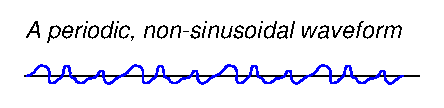
\includegraphics{vibration_17.eps}$$

An unfortunate quality of non-sinusoidal waveforms is that they do not lend themselves as readily to mathematical analysis as sinusoidal waves.  From the previous discussion on sinusoidal vibrations, we saw how simple it was to take the derivative of a sinusoidal waveform (${d \over dt} \sin \omega t = \omega \cos \omega t$), and how well this worked to predict velocity and acceleration from a function describing displacement.  Most non-sinusoidal waveforms cannot be expressed as simply and neatly as $\sin \omega t$, however, and as such are not as easy to mathematically analyze.

Fortunately, though, there is a way to represent non-sinusoidal waveforms as combinations of sinusoidal waveforms.  The French mathematician and physicist Jean Baptiste Joseph Fourier (1768-1830) proved mathematically that \textit{any} periodic waveform, no matter how strange or asymmetrical its shape may be, may be replicated by a specific sum of sine and cosine waveforms of integer-multiple frequencies.  That is, any periodic waveform (a periodic function of time, $f(\omega t)$ being the standard mathematical expression) is equivalent to a series of the following form\footnote{There is an additional term missing in this Fourier series, and that is the ``DC'' or ``bias'' term $A_0$.  Many non-sinusoidal waveforms having peak values centered about zero on a graph or oscilloscope display actually have \textit{average} values that are non-zero, and the $A_0$ term accounts for this.  However, this is usually not relevant in discussions of machine vibration, which is why I have opted to present the simplified Fourier series here.}:  \index{Fourier, Jean Baptiste Joseph}  \index{Fourier series}

$$f(\omega t) = A_1 \cos \omega t + B_1 \sin \omega t + A_2 \cos 2 \omega t + B_2 \sin 2 \omega t + \cdots A_n \cos n \omega t + B_n \sin n \omega t$$

Here, $\omega$ represents the \textit{fundamental} frequency of the waveform, while multiples of $\omega$ (e.g. $2 \omega$, $3 \omega$, $4 \omega$, etc.) represent \textit{harmonic} or \textit{overtone} frequencies of that fundamental.  The $A$ and $B$ coefficients describe the \textit{amplitudes} (heights) of each sinusoid.  We may break down a typical Fourier series in table form, labeling each term according to frequency:  \index{Harmonic frequency}  \index{Overtone frequency}  \index{Fundamental frequency}

% No blank lines allowed between lines of an \halign structure!
% I use comments (%) instead, so that TeX doesn't choke.

$$\vbox{\offinterlineskip
\halign{\strut
\vrule \quad\hfil # \ \hfil & 
\vrule \quad\hfil # \ \hfil & 
\vrule \quad\hfil # \ \hfil \vrule \cr
\noalign{\hrule}
%
% First row
\textbf{Terms} & \textbf{Harmonic} & \textbf{Overtone} \cr
%
\noalign{\hrule}
%
% Another row
$A_1 \cos \omega t + B_1 \sin \omega t$ & 1st harmonic & Fundamental \cr
%
\noalign{\hrule}
%
% Another row
$A_2 \cos 2 \omega t + B_2 \sin 2 \omega t$ & 2nd harmonic & 1st overtone \cr
%
\noalign{\hrule}
%
% Another row
$A_3 \cos 3 \omega t + B_3 \sin 3 \omega t$ & 3rd harmonic & 2nd overtone \cr
%
\noalign{\hrule}
%
% Another row
$A_4 \cos 4 \omega t + B_4 \sin 4 \omega t$ & 4th harmonic & 3rd overtone \cr
%
\noalign{\hrule}
%
% Another row
$A_n \cos n \omega t + B_n \sin n \omega t$ & $n$th harmonic & $(n-1)$th overtone \cr
%
\noalign{\hrule}
} % End of \halign 
}$$ % End of \vbox

One of the most visually convincing examples of Fourier's theorem is the ability to describe a square wave as a series of sine waves.  Intuition would suggest it is impossible to synthesize a sharp-edged waveform such as a square wave using nothing but rounded sinusoids, but it is indeed possible if one combines an \textit{infinite} series of sinusoids of successively higher harmonic frequencies, given just the right combination of harmonic frequencies and amplitudes.

\filbreak

The Fourier series for a square wave is as follows:

$$\hbox{Square wave} = 1 \sin \omega t + {1 \over 3} \sin 3 \omega t + {1 \over 5} \sin 5 \omega t + {1 \over 7} \sin 7 \omega t + \cdots$$

Such a series would be impossible to numerically calculate, but we may approximate it by adding several of the first (largest) harmonics together to see the resulting shape.  In each of the following plots, we see the individual harmonic waveforms plotted in red, with the sum plotted in blue:

$$\includegraphics{vibration_20.eps} \hskip 20pt \includegraphics{vibration_21.eps}$$

$$\includegraphics{vibration_22.eps} \hskip 20pt \includegraphics{vibration_23.eps}$$

\filbreak

If we continue this pattern up to the 13th harmonic (following the same pattern of diminishing reciprocal amplitudes shown in the Fourier series for a square wave), we see the resultant sum looking more like a square wave:

$$\includegraphics{vibration_24.eps}$$

Continuing on to the 35th harmonic, the resultant sum looks like a square wave with ripples at each rising and falling edge:

$$\includegraphics{vibration_25.eps}$$

If we were to continue adding successive terms in this infinite series, the resulting superposition of sinusoids would look more and more like a perfect square wave.

\filbreak

The only real question in any practical application is, ``What are the $A$, $B$, and $\omega$ coefficient values necessary to describe a particular non-periodic waveform using a Fourier series?''  Fourier's theorem tells us we should be able to represent \textit{any} periodic waveform -- no matter what its shape -- by summing together a particular series of sinusoids of just the right amplitudes and frequencies, but actually determining those amplitudes and frequencies is a another matter entirely.  Fortunately, modern computational techniques such as the \textit{Fast Fourier Transform} (or \textit{FFT}) algorithm make it very easy to sample any periodic waveform and have a digital computer calculate the relative amplitudes and frequencies of its constituent harmonics.  The result of a FFT analysis is a summary of the amplitudes, frequencies, and (in some cases) the phase angle of each harmonic.  \index{Fast Fourier Transform (FFT)}  \index{FFT algorithm}

To illustrate the relationship between a waveform plotted with respect to time versus a Fourier analysis showing component frequencies, I will show a pair of Fourier spectrum plots for two waveforms -- one a perfect sinusoid and the other a non-sinusoidal waveform.  First, the perfect sinusoid:

$$\includegraphics{vibration_18.eps}$$

Fourier spectra are often referred to as \textit{frequency-domain} plots because the x-axis (the ``domain'' in mathematical lingo) is frequency.  A standard oscilloscope-type plot is called a \textit{time-domain} plot because the x-axis is time.  In this first set of plots, we see a perfect sine wave reduced to a single peak on the Fourier spectrum, showing a signal with only one frequency (the fundamental, or 1st harmonic).  Here, the Fourier spectrum is very plain because there is only one frequency to display.  In other words, the Fourier series for this perfect sinusoid would be: \index{Time domain}  \index{Frequency domain}  \index{Domain, time}  \index{Domain, frequency}

$$f(\omega t) = 0 \cos \omega t + 1 \sin \omega t + 0 \cos 2 \omega t + 0 \sin 2 \omega t + \cdots 0 \cos n \omega t + 0 \sin n \omega t$$

Only the $B_1$ coefficient has a non-zero value.  All other coefficients are zero because it only takes one sinusoid to perfectly represent this waveform.

\filbreak

Next, we will examine the Fourier analysis of a non-sinusoidal waveform:

$$\includegraphics{vibration_19.eps}$$

In this second set of plots, we see the waveform is similar to a sine wave, except that it appears ``clipped'' at the peaks.  This waveform is obviously not a perfect sinusoid, and therefore cannot be described by just one of the terms ($\sin \omega t$) in a Fourier series.  It can, however, be described as equivalent to a \textit{series} of perfect sinusoids summed together.  In this case, the Fourier spectrum shows one sinusoid at the fundamental frequency, plus another (smaller) sinusoid at three times the fundamental frequency ($3 \omega$), plus another (yet smaller) sinusoid at the 5th harmonic and another (smaller still!) at the 7th: a series of \textit{odd-numbered} harmonics.

If each of these harmonics is in phase with each other\footnote{We have no way of knowing this from the Fourier spectrum plot, since that only shows us amplitude (height) and frequency (position on the x-axis).}, we could write the Fourier series as a set of sine terms:

$$f(\omega t) = (0 \hbox{ dB}) \sin \omega t + (-65 \hbox{ dB}) \sin 3 \omega t + (-95 \hbox{ dB}) \sin 5 \omega t + (-115 \hbox{ dB}) \sin 7 \omega t$$

Translating the decibel amplitude values into simple coefficients, we can see just how small these harmonic sinusoids are in comparison to the fundamental:

$$f(\omega t) = 1 \sin \omega t + 0.000562 \sin 3 \omega t + 0.0000178 \sin 5 \omega t + 0.00000178 \sin 7 \omega t$$

If the waveform deviated even further from a perfect sinusoid, we would see a Fourier spectrum with taller harmonic peaks, and perhaps more of them (possibly including some even-numbered harmonics, not just odd-numbered), representing a harmonically ``richer'' spectrum.

Within the technical discipline of machine vibration analysis, harmonic vibrations are often referred to by labels such as \textit{1X}, \textit{2X}, and \textit{3X}, the integer number corresponding to the harmonic order of the vibration.  The fundamental, or first harmonic, frequency of a vibration would be represented by ``1X'' while ``2X'' and ``3X'' represent the second- and third-order harmonic frequencies, respectively.

\vskip 10pt

On a practical note, the Fourier analysis of a machine's vibration waveform holds clues to the successful balancing of that machine.  A first-harmonic vibration may be countered by placing an off-center mass on the rotating element 180 degrees out of phase with the offending sinusoid.  Given the proper phase (180$^{o}$ -- exactly opposed) and magnitude, any harmonic may be counterbalanced by an off-center mass rotating at the same frequency.  In other words, we may cancel any particular harmonic vibration with an equal and opposite harmonic vibration.

If you examine the ``crankshaft'' of a piston engine, for example, you will notice counterweights with blind holes drilled in specific locations for balancing.  These precisely-trimmed counterweights compensate for first-harmonic (fundamental) frequency vibrations resulting from the up-and-down oscillations of the pistons within the cylinders.  However, in some engine designs such as inline 4-cylinder arrangements, there are significant harmonic vibrations of greater order than the fundamental, which \textit{cannot} be counterbalanced by any amount of weight, in any location, on the rotating crankshaft.  The reciprocating motion of the pistons and connecting rods produce periodic vibrations that are non-sinusoidal, and these vibrations (like all periodic, non-sinusoidal waveforms) are equivalent to a series of harmonically-related sinusoidal vibrations.

Any weight attached to the crankshaft will produce a first-order (fundamental) sinusoidal vibration, and that is all.  In order to counteract harmonic vibrations of higher order, the engine requires counterbalance shafts spinning at speeds corresponding to those higher orders.  This is why many high-performance inline 4-cylinder engines employ counterbalance shafts spinning at \textit{twice} the crankshaft speed: to counteract the second-harmonic vibrations created by the reciprocating parts.  If an engine designer were so inclined, he or she could include several counterbalance shafts, each one spinning at a different multiple of the crankshaft speed, to counteract as many harmonics as possible.  At some point, however, the inclusion of all these shafts and the gearing necessary to ensure their precise speeds and phase shifts would interfere with the more basic design features of the engine, which is why you do not typically see an engine with multiple counterbalance shafts.

\vskip 10pt

The harmonic content of a machine's vibration signal in and of itself tells us little about the health or balance of that machine.  It may be perfectly normal for a machine to have a very ``rich'' harmonic signature due to convoluted motions of its parts\footnote{Machines with reciprocating components, such as pistons, cam followers, poppet valves, and such are notorious for generating vibration signatures which are anything but sinusoidal even under normal operating circumstances!}.  However, Fourier analysis provides a simple way to quantify complex vibrations and to archive them for future reference.  For example, we might gather vibration data on a new machine immediately after installation (including its Fourier spectra on all vibration measurement points) and save this data for safe keeping in the maintenance archives.  Later, if and when we suspect a vibration-related problem with this machine, we may gather new vibration data and compare it against the original ``signature'' spectra to see if anything substantial has changed.  Changes in harmonic amplitudes and/or the appearance of new harmonics may point to specific problems inside the machine.  Expert knowledge is usually required to interpret the spectral changes and discern what those specific problem(s) might be, but at least this technique does have diagnostic value in the right hands.

% ADD: sidebands caused by amplitude modulation of gear or bearing noise










\filbreak
\section{Vibration sensors}

Sensors used to measure vibration come in three basic types: \textit{displacement}, \textit{velocity}, and \textit{acceleration}.  Displacement sensors measure changes in distance between a machine's rotating element and its stationary housing (frame).  Displacement sensors come in the form of a probe that threads into a hole drilled and tapped in the machine's frame, just above the surface of a rotating shaft.  Velocity and acceleration sensors, by contrast, measure the velocity or acceleration of whatever element the sensor is attached to, which is usually some external part of the machine frame\footnote{From the perspective of measurement, it would be ideal to affix a velocimeter or accelerometer sensor directly to the rotating element of the machine, but this leads to the problem of electrically connecting the (now rotating!) sensor to stationary analysis equipment.  Unless the velocity or acceleration sensor is wireless, the only practical mounting location is on the stationary frame of the machine.}.

$$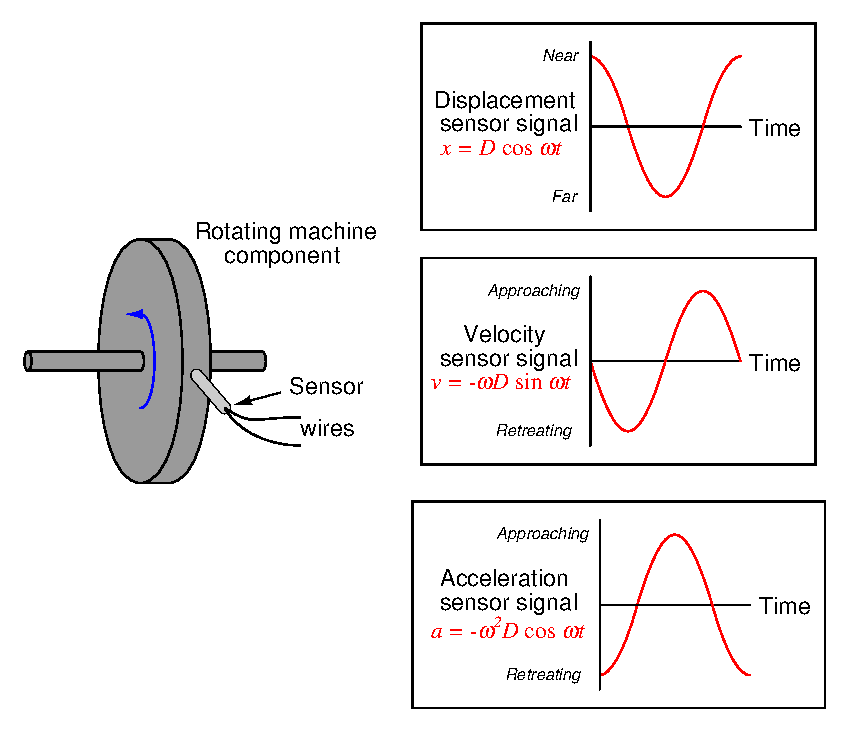
\includegraphics{vibration_02.eps}$$

A design of displacement sensor manufactured by the Bently-Nevada corporation uses electromagnetic \textit{eddy current} technology to sense the distance between the probe tip and the rotating machine shaft.  The sensor itself is an encapsulated coil of wire, energized with high-frequency alternating current (AC).  The magnetic field produced by the coil induces eddy currents in the metal shaft of the machine, as though the metal piece were a short-circuited secondary coil of a transformer (with the probe's coil as the transformer primary winding).  The closer the shaft moves toward the sensor tip, the tighter the magnetic coupling between the shaft and the sensor coil, and the stronger the eddy currents.  \index{Bently-Nevada vibration monitoring equipment}

The high-frequency oscillator circuit providing the sensor coil's excitation signal becomes loaded by the induced eddy currents.  Therefore, the oscillator's load becomes a direct indication of how close the probe tip is to the metal shaft.  This is not unlike the operation of a metal detector: measuring the proximity of a wire coil to any metal object by the degree of loading caused by eddy current induction.

In the Bently-Nevada design, the oscillator circuit providing sensor coil excitation is called a \textit{proximitor}.  The proximitor module is powered by an external DC power source, and drives the sensor coil through a coaxial cable.  Proximity to the metal shaft is represented by a DC voltage output from the proximitor module, with 200 millivolts per mil (1 mil = $1 \over 1000$ inch) of motion being the standard calibration.  \index{Proximitor, Bently-Nevada}

$$\includegraphics{vibration_05.eps}$$

Since the proximitor's output voltage is a direct representation of distance between the probe's tip and the shaft's surface, a ``quiet'' signal (no vibration) will be a pure DC voltage.  The probe is adjusted by a technician such that this quiescent voltage will lie between the proximitor's output voltage range limits.  Any vibration of the shaft will cause the proximitor's output voltage to vary in precise step.  A shaft vibration of 28.67 Hz, for instance, will cause the proximitor output signal to be a 28.67 Hz waveform superimposed on the DC ``bias'' voltage set by the initial probe/shaft gap.

An oscilloscope connected to this output signal will show a direct representation of shaft vibration, as measured in the axis of the probe.  In fact, \textit{any} electronic test equipment capable of analyzing the voltage signal output by the proximitor may be used to analyze the machine's vibration: oscilloscopes, spectrum analyzers, peak-indicating voltmeters, RMS-indicating voltmeters, etc.

\filbreak

Photographs of a Bently-Nevada displacement sensor (sensing axial vibration on a ``ring'' style air compressor) and two proximitor modules are shown here:

$$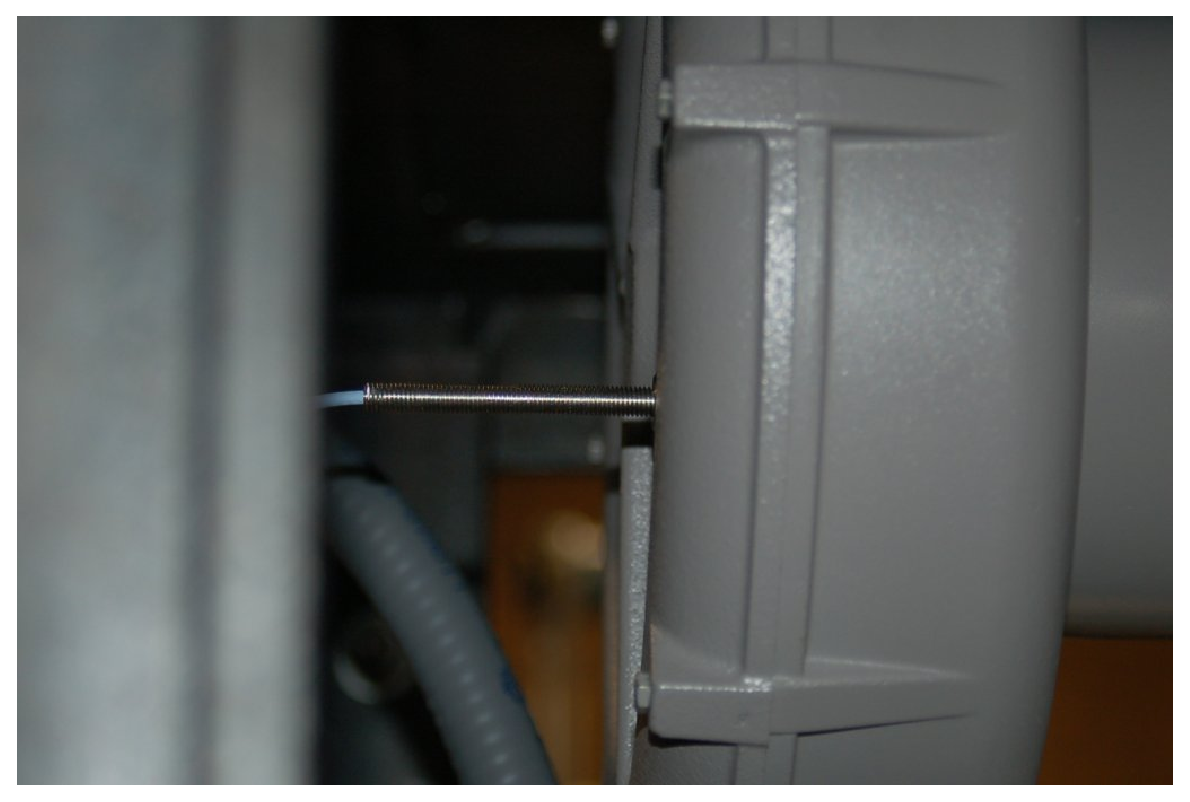
\includegraphics[width=2.5in]{vibration_10.eps} \hskip 30pt 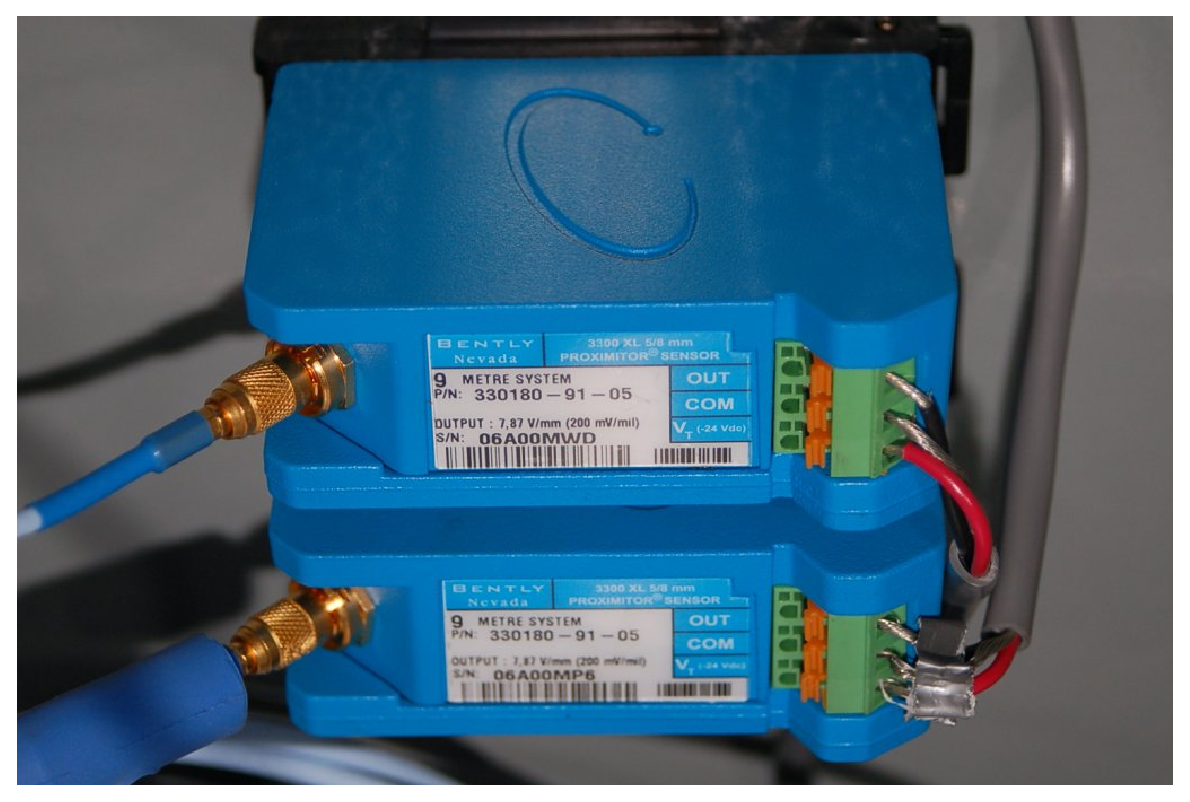
\includegraphics[width=2.5in]{vibration_11.eps}$$

\filbreak

It is customary to arrange a set of three displacement probes at the end of a machine shaft to measure vibration: two \textit{radial} probes and one \textit{axial} (or \textit{thrust}) probe.  The purpose of this \textit{triaxial} probe configuration is to measure shaft vibration (and/or shaft displacement) in all three dimensions:  \index{Triaxial vibration probe array}

$$\includegraphics{vibration_06.eps}$$

The following photograph shows two displacement probes sensing vibration in the X and Y radial axes for a large vertical-shaft hydroelectric power plant turbine at Grand Coulee Dam:

$$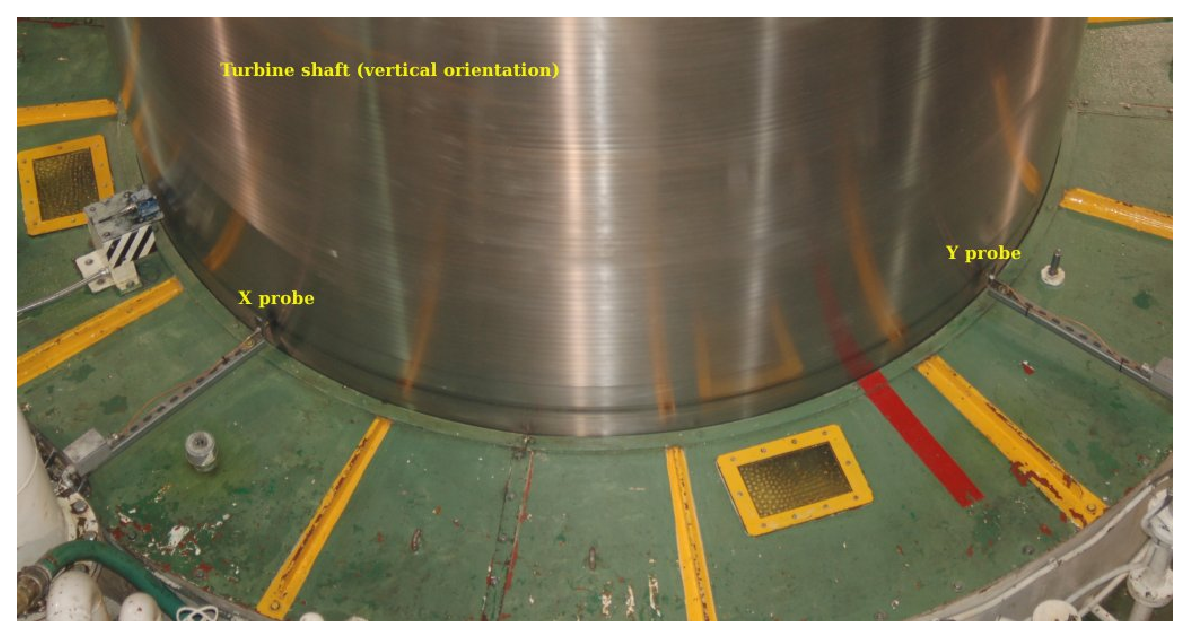
\includegraphics[width=6in]{vibration_30.eps}$$

\filbreak

It is also common to see one \textit{phase reference} probe installed on the machine shaft, positioned in such a way that it detects the periodic passing of a keyway or other irregular feature on the shaft.  The ``keyphasor'' signal will consist of one large pulse per revolution:  \index{Phase reference signal, vibration monitoring}  \index{Keyphasor}

$$\includegraphics{vibration_09.eps}$$

The purpose of a keyphasor signal is two-fold: to provide a reference point in the machine's rotation to correlate other vibration signals against, and to provide a simple means of measuring shaft speed.  The location in time of the pulse represents shaft position, while the frequency of that pulse signal represents shaft speed.  

For instance, if one of the radial displacement sensors indicates a high vibration at the same frequency as the shaft rotation (i.e. the shaft is bowed in one direction, like a banana spinning on its long axis), the phase shift between the vibration's sinusoidal peak and the phase reference pulse will indicate to maintenance machinists where the machine is out of balance.  This is not unlike automatic tire-balancing machines designed to measure imbalance in automobile tire and wheel assemblies: the machine must have some way of indicating to the human operator \textit{where} a balancing weight should be placed, not just how far out of balance the tire is.  In the case of machine vibration monitoring equipment, the keyphasor signal and one of the axial displacement signals may be simultaneously plotted on a dual-trace oscilloscope for the purposes of determining the position of the imbalance on the machine shaft.











\filbreak
\section{Monitoring hardware}

The following photograph shows a large air blower in a wastewater treatment facility equipped with a Bently-Nevada model 3300 vibration monitoring rack (located left-center on the foreground panel):  \index{Bently-Nevada model 3300 vibration monitor}

$$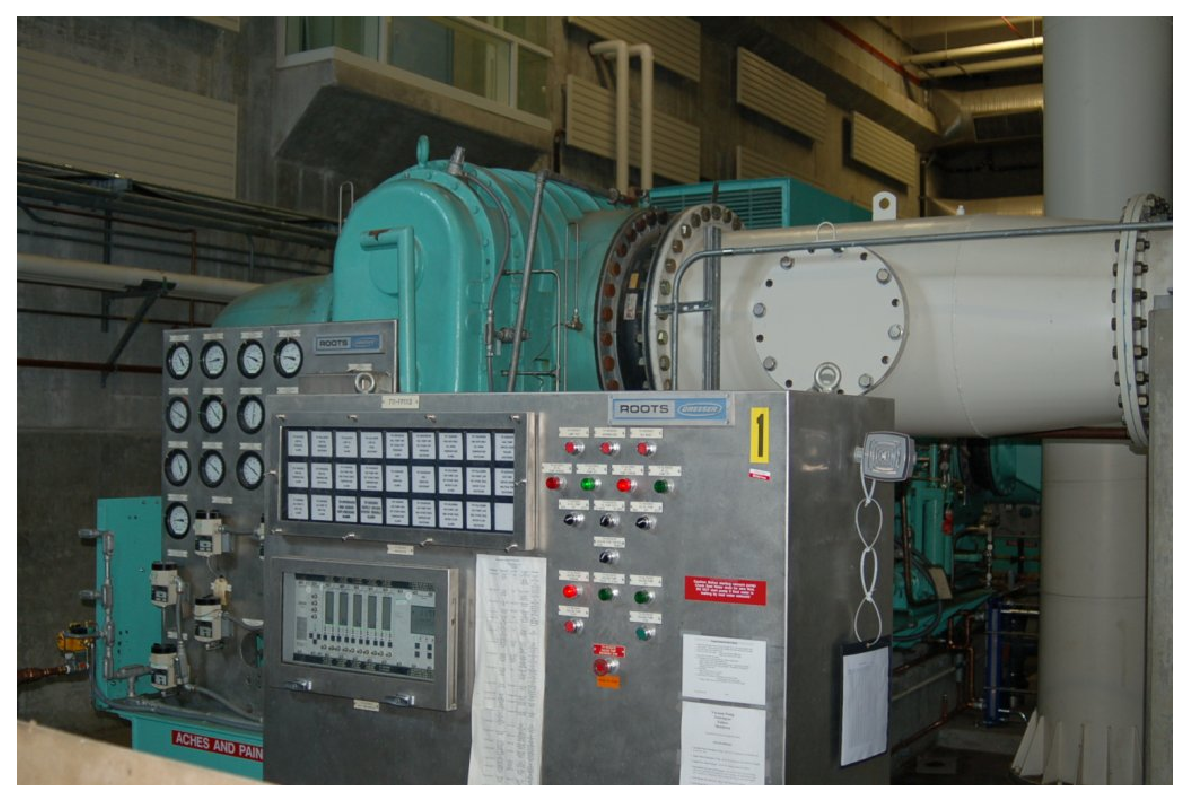
\includegraphics[width=4in]{vibration_07.eps}$$

Five vibration measurement and display cards are installed in this rack, each card capable of processing up to two displacement sensor signals.  A six-channel temperature monitor card is also installed in the rack, used to display bearing and other machine component temperatures.  Like the vibration cards, the temperature card is capable of generating both ``alert'' and ``trip'' signals, monitoring the presence of slightly abnormal conditions and taking automatic shut-down action in the event of excessively abnormal conditions, respectively.

A closer view of a different Bently-Nevada model 3300 vibration monitoring rack is shown in this photograph:

$$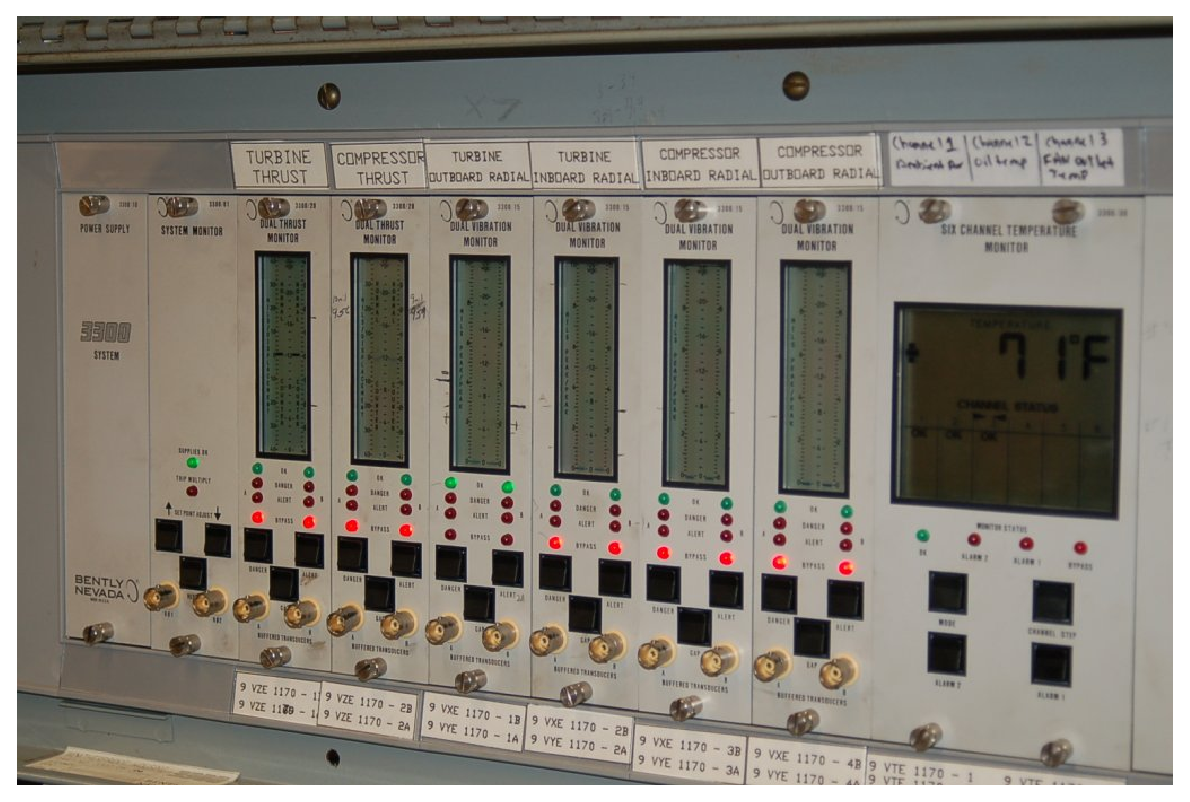
\includegraphics[width=3in]{vibration_12.eps}$$

Each ``card'' inserted into this rack performs a different measurement function.

\filbreak

The following photographs show even closer views of the cards, revealing the display bargraphs and the units of measurement.  From left to right; thrust measurement, vibration measurement, temperature measurement (6 channels), and speed measurement:

$$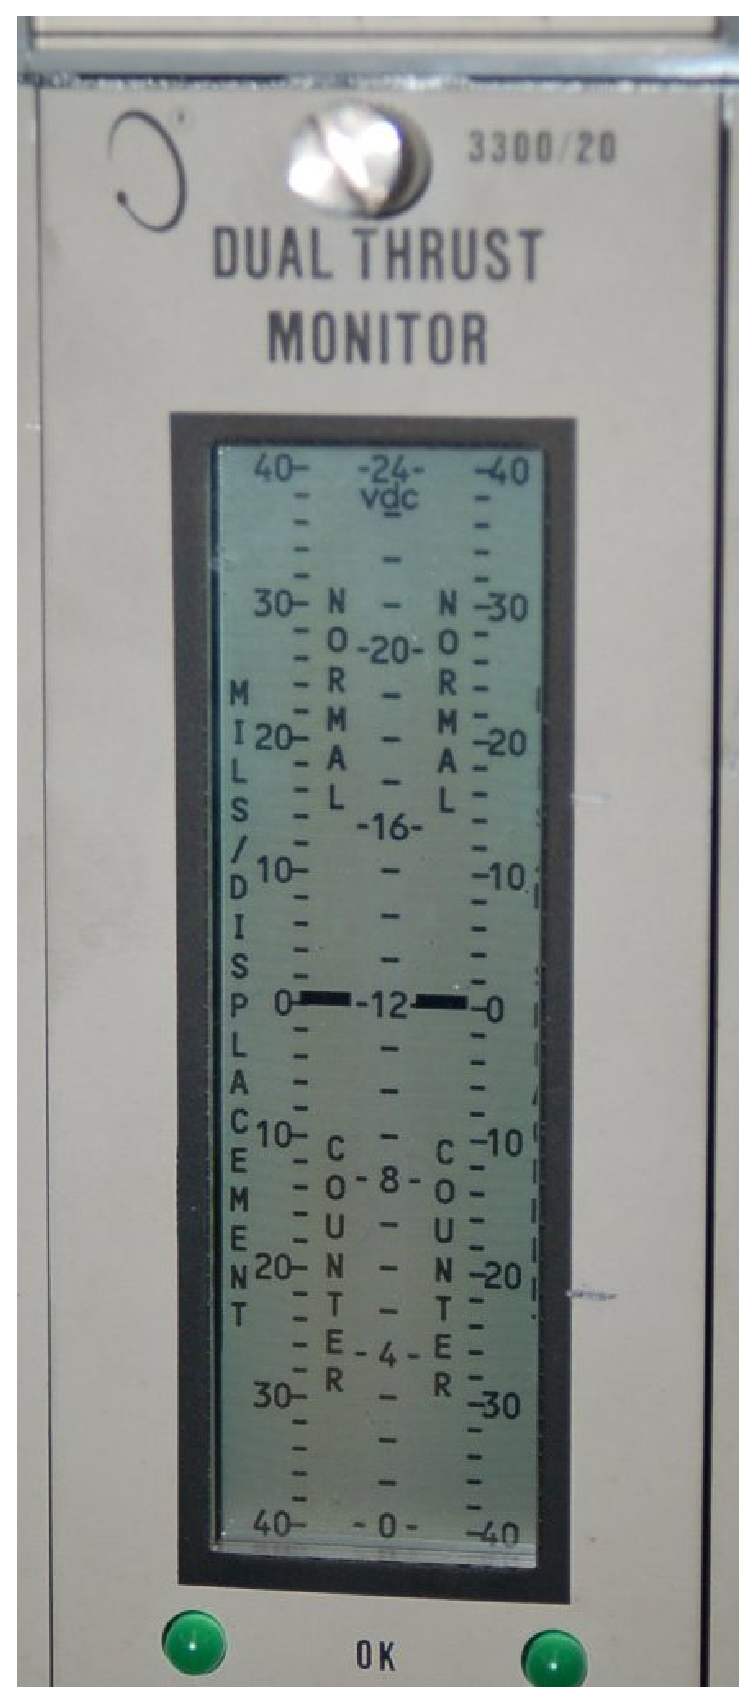
\includegraphics[height=3in]{vibration_13.eps} \hskip 20pt 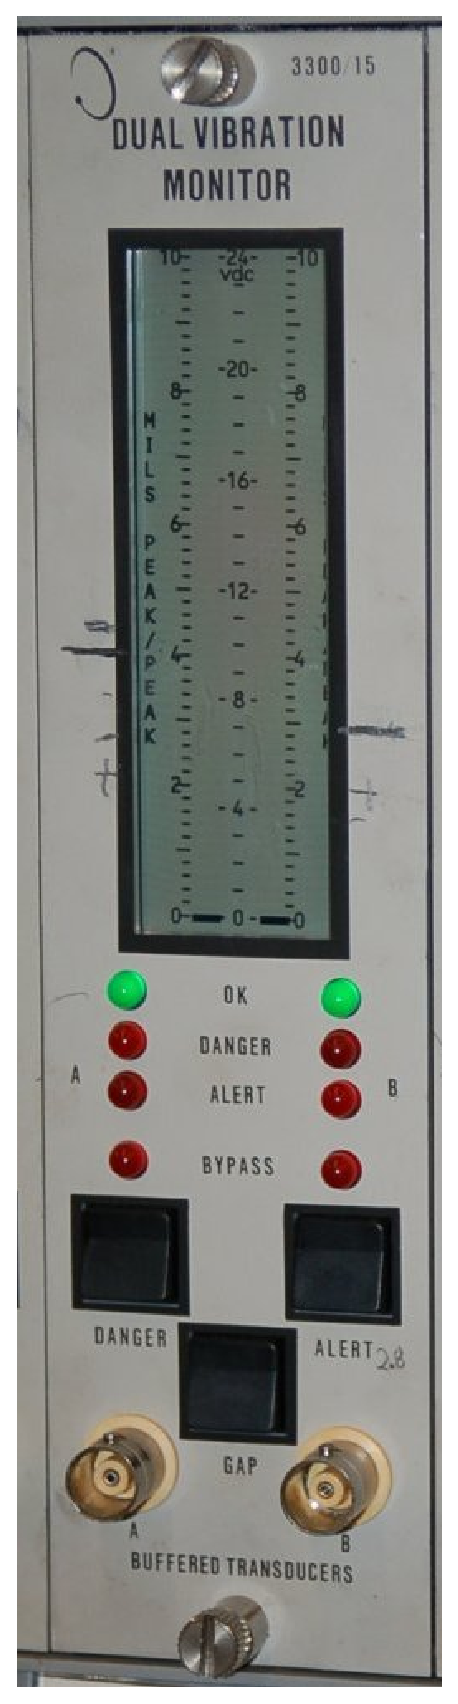
\includegraphics[height=3in]{vibration_14.eps} \hskip 20pt 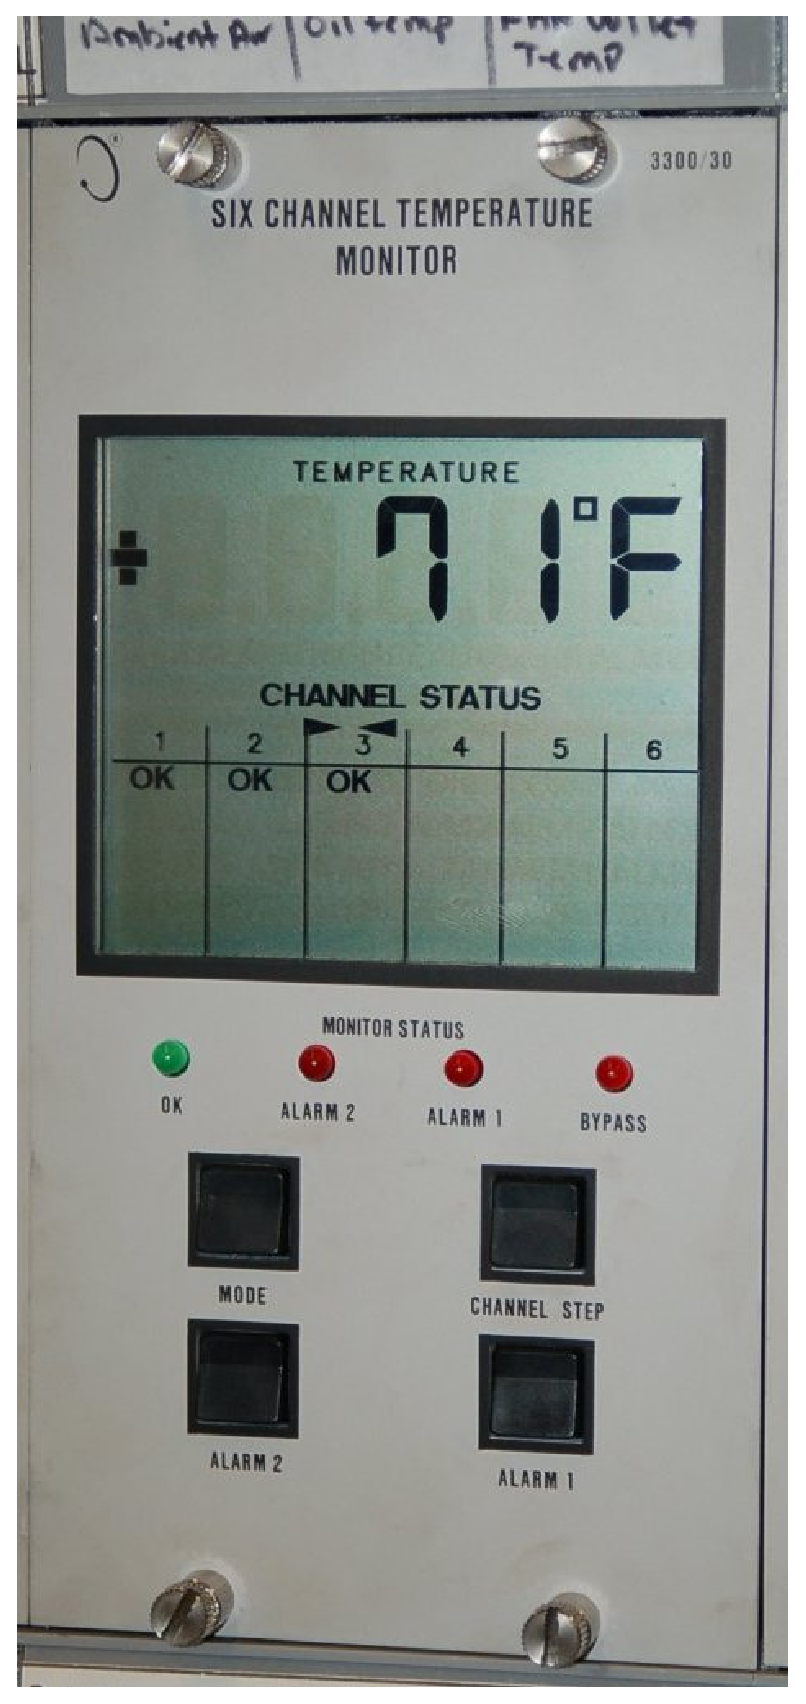
\includegraphics[height=3in]{vibration_15.eps} \hskip 20pt 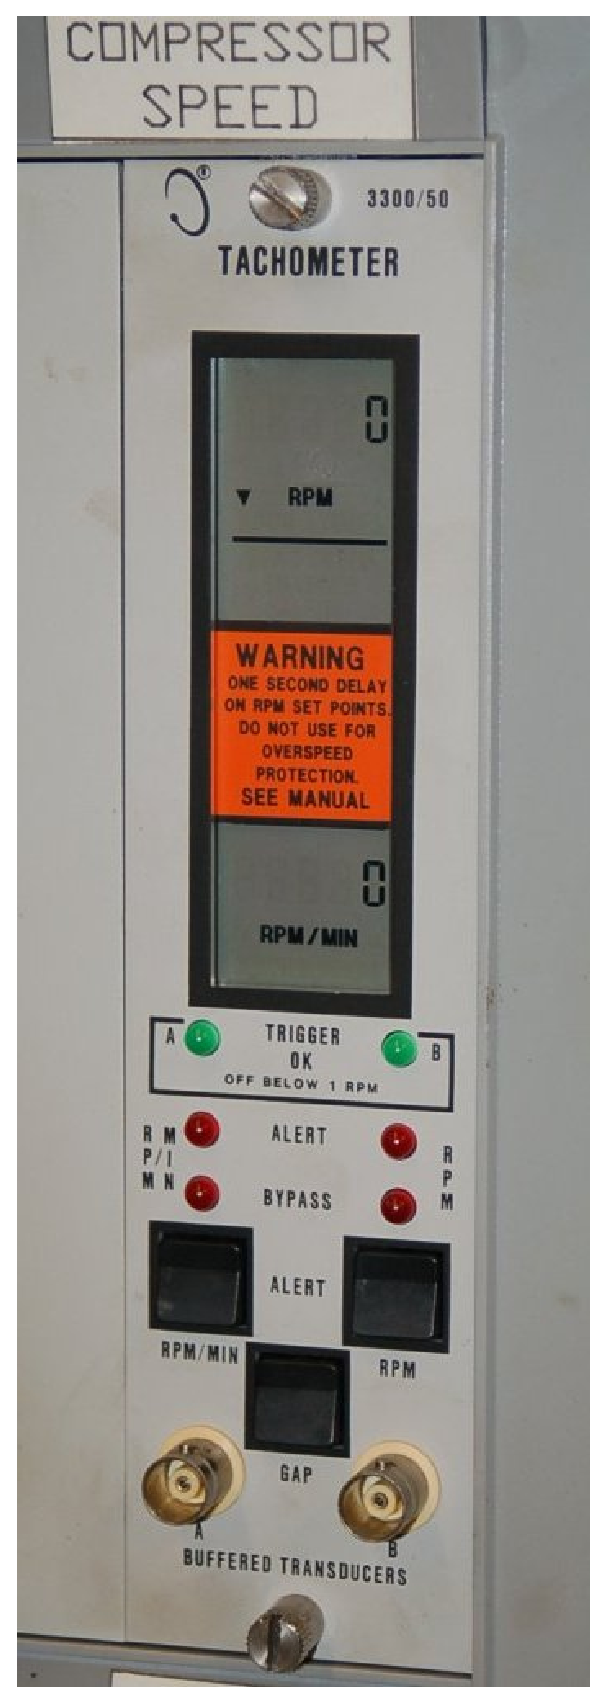
\includegraphics[height=3in]{vibration_16.eps}$$

BNC-style cable connectors on the front of the cards provide convenient connection points for electronic test equipment such as oscilloscopes or spectrum analyzers.  This eliminates the need to un-do wire connections on the proximitor units in order to take diagnostic measurements.  Each card also provides ``alert'' and ``danger'' levels for their respective measurements, generating a contact-closure signal which may be connected to an automatic shutdown (``trip'') system to take protective action if vibration or thrust displacement ever exceeds pre-set limits.  \index{BNC style connector}

\filbreak

Another variety of vibration monitoring hardware is the Bently-Nevada 1701 FieldMonitor.  This hardware lacks the convenient front-panel displays of the model 3300, opting instead to communicate vibration data in digital form to an Allen-Bradley programmable logic controller (PLC).  Not only does this make it possibly to display the vibration data remotely through HMI (Human-Machine Interface) panels, but it also enables vibration data to engage automatic ``trip'' logic programming in the PLC to shut the machine down in the event of excessive vibration.  This next photograph shows several FieldMonitor modules plugged into a rack, acquiring displacement data from eight proximity probes (X and Y axis radial measurements at three machine bearing locations, plus one axial (thrust) measurement and one phase reference measurement):  \index{Bently-Nevada model 1701 FieldMonitor vibration monitor}

$$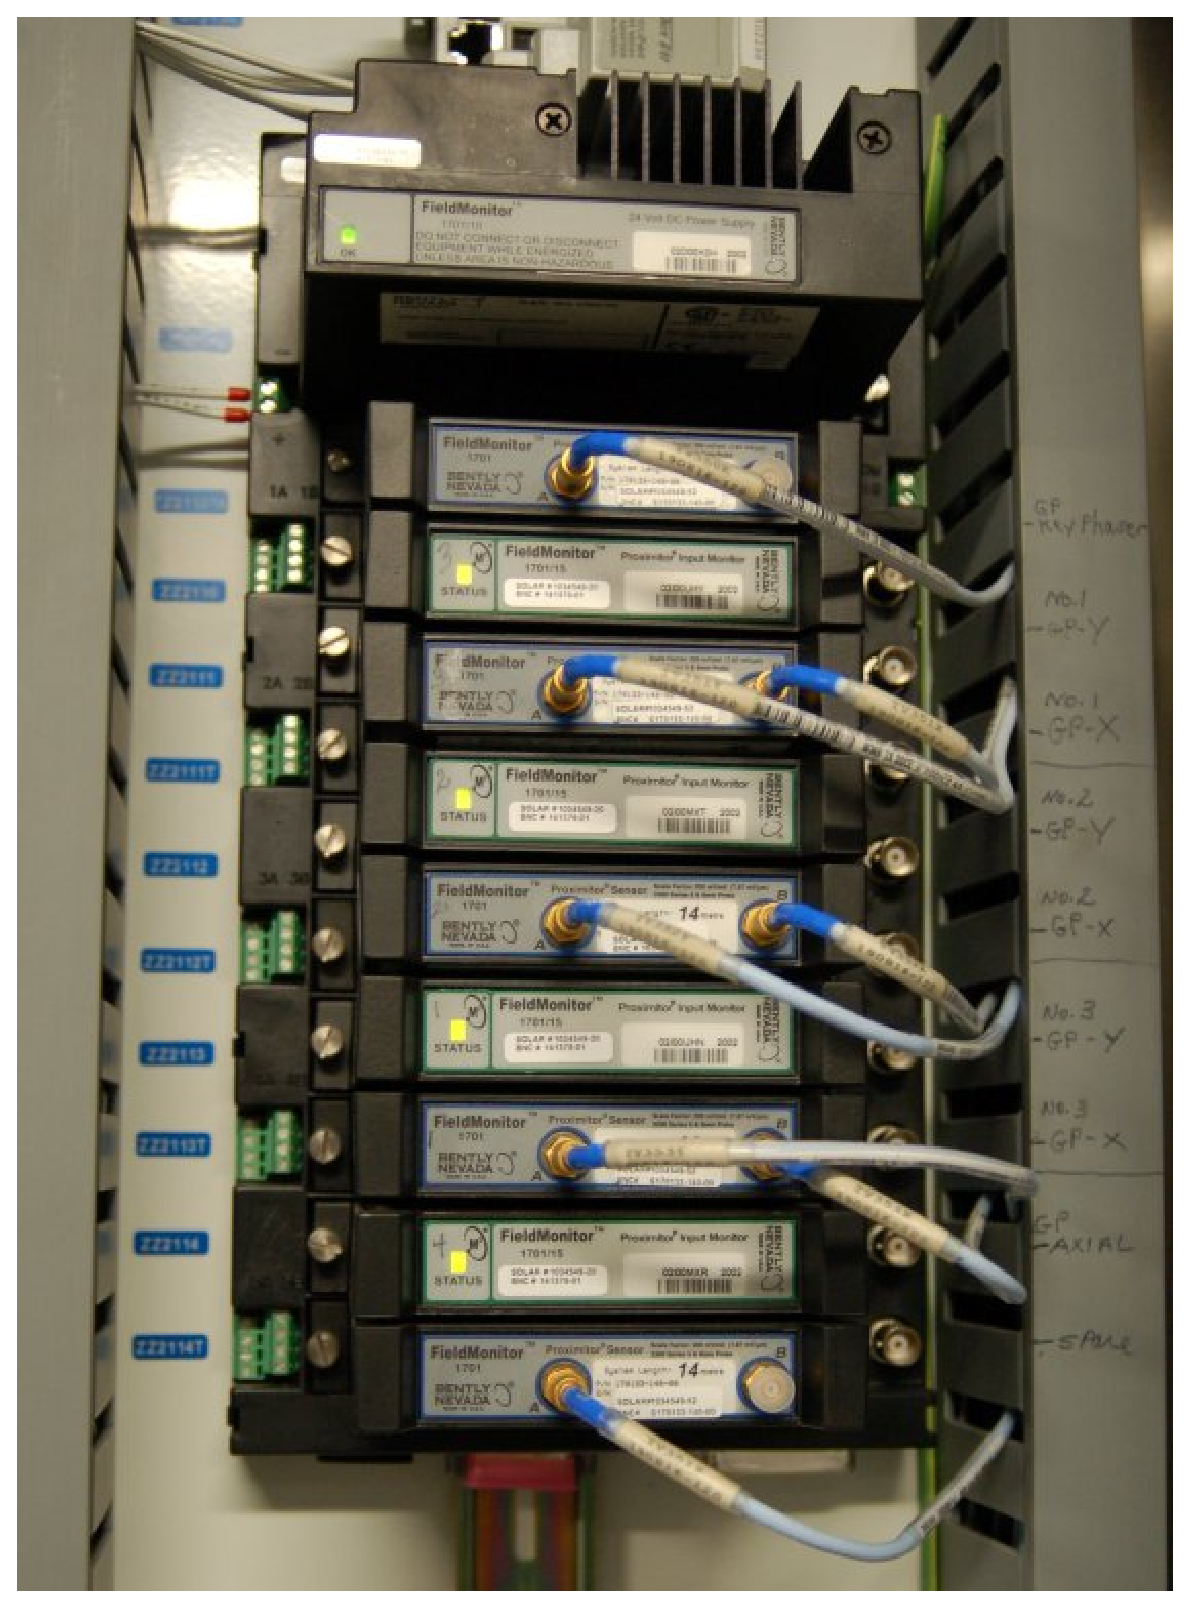
\includegraphics[width=3in]{vibration_08.eps}$$












\filbreak
\section{Mechanical vibration switches}

A much simpler alternative to continuous vibration sensors (displacement or acceleration) and monitoring equipment suitable for less critical applications is a simple mechanical switch actuated by a machine's vibration.  These switches cannot, of course, quantitatively analyze machine vibrations, but they do serve as qualitative indicators of gross vibration.  

The following photograph shows a Robertshaw ``Vibraswitch'' unit:  \index{Robertshaw Vibraswitch}

$$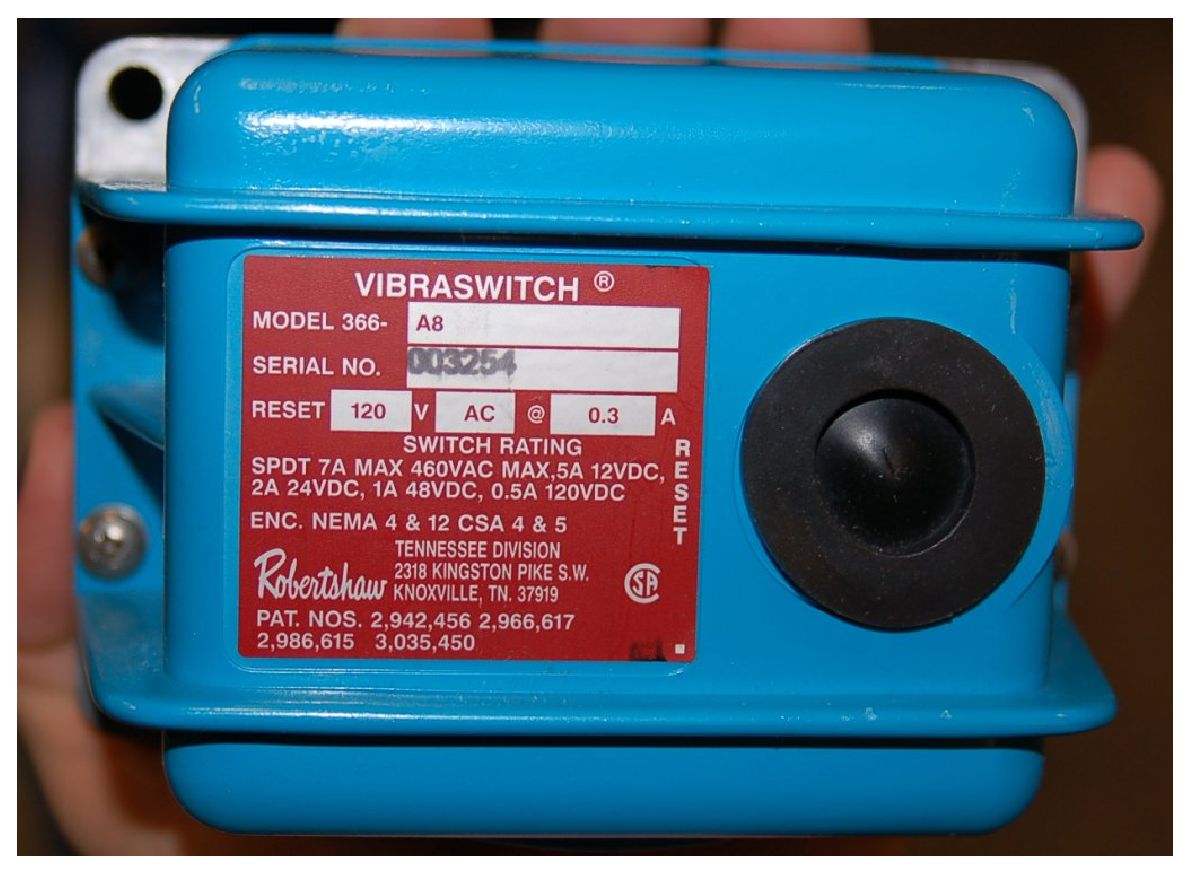
\includegraphics[width=4in]{vibration_26.eps}$$

\filbreak

This switch works on the principle of a weighted lever generating a force when shaken.  A pair of magnets located at the weighted end of the lever hold it in either the ``reset'' (normal) or ``tripped'' position:  \index{Normal state of a vibration switch}

$$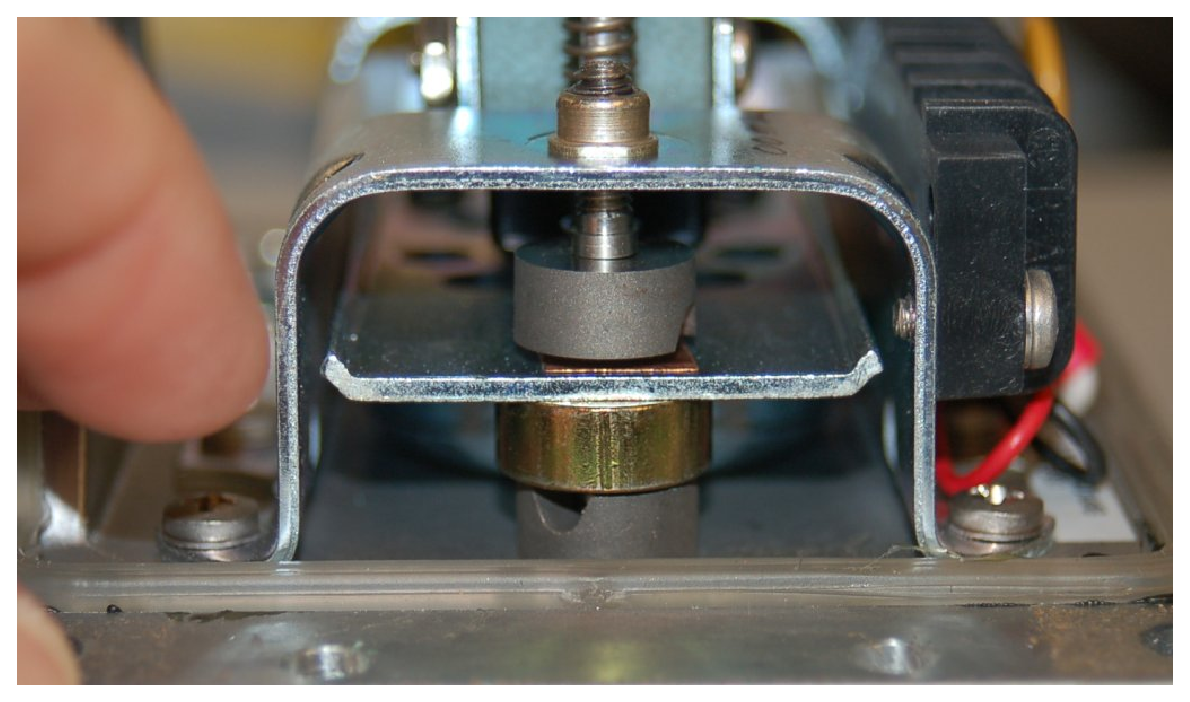
\includegraphics[width=2.5in]{vibration_27.eps} \hskip 30pt 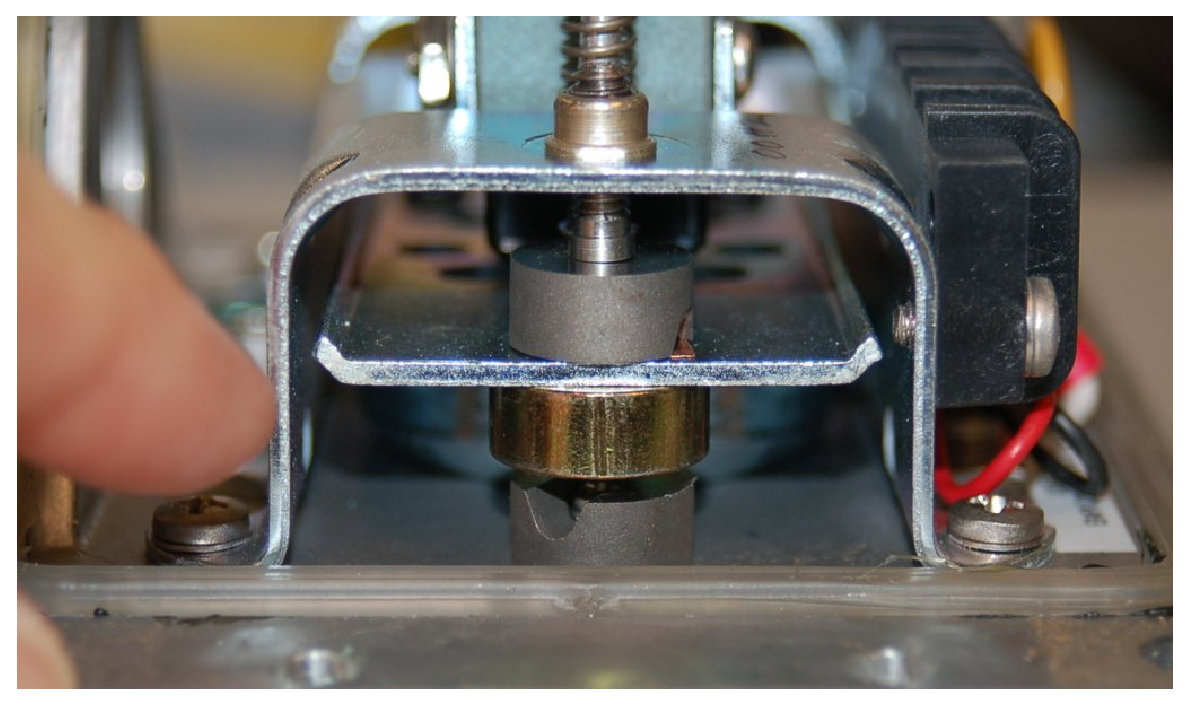
\includegraphics[width=2.5in]{vibration_28.eps}$$

When reset, the lever is pre-loaded by spring tension to flip to the ``tripped'' position.  All it needs to make that transition is enough acceleration to generate the ``breakaway'' force necessary to pull away from the holding magnet.  Once the acceleration force exceeds that threshold, the lever moves toward the other magnet, which holds it securely in position so that switch will not ``reset'' itself with additional vibration.

\filbreak

This pre-loading spring is adjustable by a small screw, making it possible to easily vary the sensitivity of the switch:

$$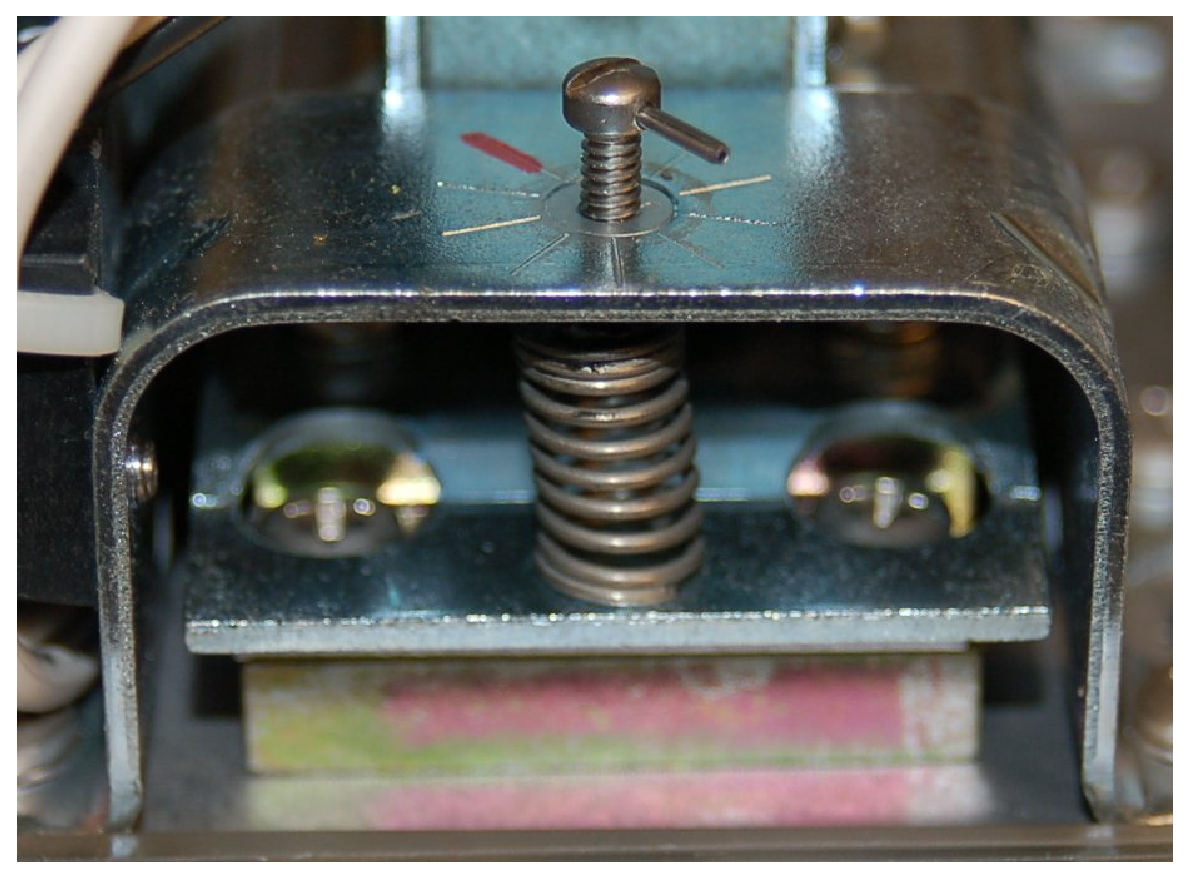
\includegraphics[width=3in]{vibration_29.eps}$$








\filbreak
\section{Review of fundamental principles}

Shown here is a partial listing of principles applied in the subject matter of this chapter, given for the purpose of expanding the reader's view of this chapter's concepts and of their general inter-relationships with concepts elsewhere in the book.  Your abilities as a problem-solver and as a life-long learner will be greatly enhanced by mastering the applications of these principles to a wide variety of topics, the more varied the better.

\begin{itemize}
\item \textbf{Newton's Second Law of motion}: $F = ma$, describing how the acceleration of an object is directly proportional to the amount of applied (resultant) force and inversely proportional to its mass.  Relevant to the calculation of force developed on a machine part from the acceleration and deceleration of vibration.
\item \textbf{Differentiation (calculus)}: where one variable is proportional to the rate-of-change of two others.  Differentiation always results in a division (quotient) of units.  Relevant to conversion from position to velocity, and from velocity to acceleration: $v = {dx \over dt}$ and $a = {dv \over dt}$.
\item \textbf{Integration (calculus)}: where one variable is proportional to the accumulation of the product of two others.  Integration always results in a multiplication of units.  Relevant to conversion from acceleration to velocity, and from velocity to position: $v = \int a \> dt$ and $x = \int v \> dt$.  
\item \textbf{Fourier transforms}: any repetitive waveform, no matter what its shape, is mathematically equivalent to a series of sinusoidal (sine and cosine) waves of different frequencies, amplitudes, and phase shifts added together.  The frequencies of these sinusoids are all integer multiples, called harmonics.  Relevant to decomposing vibrational wave signals into their constituent harmonic frequencies, to determine which parts of a machine are vibrating most.
\end{itemize}







\filbreak
\section*{References}

% In alphabetical order!
% \noindent
% Lastname, Firstname MiddleI., \textit{Book Title}, Publisher, City, State, Year.
% \vskip 10pt
% \noindent
% Lastname, Firstname MiddleI., \textit{Book Title}, Publisher, City, State, Year.
% etc . . .

\noindent
Kaplan, Wilfred, \textit{Advanced Mathematics for Engineers}, Addison-Wesley Publishing Company, Reading, MA, 1981.

\vskip 10pt

\noindent
Smith, Steven W., \textit{The Scientist and Engineer's Guide to Digital Signal Processing}, California Technical Publishing, San Diego, CA, 1997.

\vskip 10pt

\noindent
White, Glenn D., \textit{Introduction to Machine Vibration}, version 1.76, part number 8569, DLI Engineering Corp., Bainbridge Island, WA, 1995.













%%%%%%%%%%%%%%%%%%%%%%%%%%%%%%%%%%%%%%%%%%%%%%%%%%%%

